\appendices

\section{Generation Prompts and Recorded Settings}

\label{app:prompts}

The supplement gives the original Chinese prompt templates, SHA-256 hashes,
and English translations. The descriptions below explain each task in
simple English. Saved records contain parsed responses and removed spans.
The original templates remain in the experiment archive.

\subsection{Deletion Completion Prompt}

\label{app:prompt_deletion}

The deletion prompt asks the model to read the original and changed
service document. It asks for rule information from the removed phrases
and reusable graph constraints. The response must follow the supplied
JSON format. Inputs include the service item, original text, changed text,
and removed spans. Candidates use general types and relations.

The JSON fields are \texttt{strategy}, \texttt{service\_item},
\texttt{analysis}, \texttt{removed\_fragments},
\texttt{missing\_rule\_candidates}, and \texttt{proposed\_rules}.
The last field contains the seven categories below.
The runner makes one call per document and strategy.

\subsection{Augmentation Expansion Prompt}

\label{app:prompt_augmentation}

The augmentation prompt asks for up to three reasonable extra sentences
for the service document. It then asks for reusable graph rules from
these additions. The response must follow the supplied JSON format.
Inputs include the service item and original text.

Its fields are \texttt{strategy}, \texttt{service\_item}, \texttt{analysis},
\texttt{added\_clauses}, and \texttt{proposed\_rules}.
Both prompts share seven categories: entity types, relation types,
forbidden patterns, allowed patterns, hierarchy statements,
geographical hierarchy patterns, and statements about required steps.

\subsection{Defaults and Recorded Settings}

The script defaults to Qwen3-32B and temperature 0.2.
It removes up to five spans of at most six characters and requests
up to three extra sentences. The client leaves the completion limit
and top-$p$ unset. Historical records store document ID, service item,
strategy, parsed result, and removed spans when present.
Full per-call settings and rendered requests are absent from these logs.
The separate 45-document extraction test records Qwen3.8-27B-no-thinking.

\section{RuleTest-94 and Direct Execution}

\label{app:testset}

RuleTest-94 has 30 clean and 64 defective records: 10 hierarchy reversals,
10 absurd relations, 10 reverse-supervision cases, 30 required-step or
missing-field cases, and four specialist cases. The scorer reads
\texttt{expected\_detection}. A \texttt{pass} label is negative;
\texttt{fail} and \texttt{specialist\_miss} are positive.
The suite provides these designed labels.

The union of hand-written family checks detects all 64 defects and flags
zero clean records. Its precision Wilson interval is $[0.943,1.000]$;
specificity is $[0.886,1.000]$. Section~\ref{sec:rule_execution_audit}
gives direct execution of saved candidates.

\label{app:rule_format}

Each compiled rule has an ID, allowed or forbidden kind, exact
subject-type/relation/object-type pattern, and original source positions.
Exact pattern matches decide which records it covers.
Permissions allow a combination. Prohibitions flag it.
A conflict causes a skipped decision. The log retains unsupported
natural-language candidates.

\section{Document Pilot with Given Types}

\label{app:docred_pilot}

We split source-grouped DocRED~\cite{ref_docred} documents into 180 training,
60 development, and 60 test items from the original annotated training
set. Entity IDs and mention types are given. Public source inputs and
reference relations are stored apart.

Ten fixed development documents each receive two rule responses and one
extraction response from Gemma. The 30 outputs use 34 requests including
retries. All twenty rule responses parse. They give 263 compiled candidates:
156 allowed and 107 forbidden patterns. One extraction fails the fixed
parser and becomes an empty graph. The other outputs give 106 executable
relations. Five two-document episodes run stop and four acquisition/repair
schedules. All schedules remove zero records and reach the same final
graph within each episode. The generated forbidden rules thus match zero
repair targets in these outputs. Records and code are in
\texttt{exps/paper2\_docred}.

\subsection{Source-Rule Development Test}

\label{app:docred_v2}

This version keeps the two prompts and four-action scheduler and adds
source rules for each document. A candidate marks a record as supported,
contradicted, or insufficient. The compiler checks an exact quote in
an original numbered sentence and saves character positions.
Augmentation sentences serve as generation hints. Insufficient evidence
or conflicting support and contradiction cause a skipped decision.
An allowed type rule leaves a source contradiction active.

Let $V(g;R)$ be the set of nonconflicting violations. Let $N$ be the
initial record count, using one for an empty input.
We use $G(g;R)=1-|V(g;R)|/N$ and coverage $C$ over initial records.
The graph-change term checks both graphs under updated rules:

\begin{align}
r_t={}&0.5\left[G(g_{t+1};R_{t+1})-G(g_t;R_{t+1})\right] \nonumber\\
&+0.5(C_{t+1}-C_t)-0.004a_t \nonumber\\
&-0.00002d_t-|V_{\mathrm{edit},t}|/N,
\end{align}

Here $a_t$ counts acquired responses and $d_t$ counts removed records.
$V_{\mathrm{edit},t}=V(g_{t+1};R_{t+1})\setminus V(g_t;R_{t+1})$ counts
edit-created violations. Acquisition can reveal an existing violation
with zero charge for creating it. A two-record synthetic test changes
discounted acquire--repair return from $-0.266519$ to $0.483481$
at discount $0.95$. This test checks reward accounting. The model judges
source support; the compiler checks the quote text.

Before calls, we fix the first ten development pairs, or 20 documents.
Each pair has one reference graph and one reference graph with added
endpoint or relation changes. The added count is $\lceil0.2|G^*|\rceil$.
References supply input construction and scoring. Prompts and policies
use public inputs. Each observation has 14 summaries and an action mask.
An episode allows four responses, two per strategy, and ten steps.
The removal guard blocks actions that would empty a nonempty graph.

\begin{table}[t]
\centering
\caption{Source-rule test on ten fixed document pairs. F1 and facts kept are episode means. Lost counts removed reference facts. Schedules are fixed.}
\label{tab:docred_source_pilot}
\small
\begin{tabular}{lrrr}
\hline
Schedule & F1 (\%) & Facts kept (\%) & Lost \\
\hline
Stop & 94.42 & 100.00 & 0 \\
Acquire then repair & 94.59 & 98.34 & 4 \\
Repair when feasible & 91.63 & 93.51 & 18 \\
Uniform feasible & 94.42 & 100.00 & 0 \\
\hline
\end{tabular}
\end{table}

The 40 outputs use 40 Gemma requests. They compile to 357 type rules,
61 source-support rules, and 6 source-contradiction rules.
Source rules trigger removal in 4 of ten episodes. The fixed expansion
check requires at least two such episodes, higher mean reference F1,
and at least 99\% reference facts kept. This version ends at that check.
Scores measure reference recovery and injected-item removal.
Saved-output replay uses zero API calls.

\begin{figure*}[t]
\centering
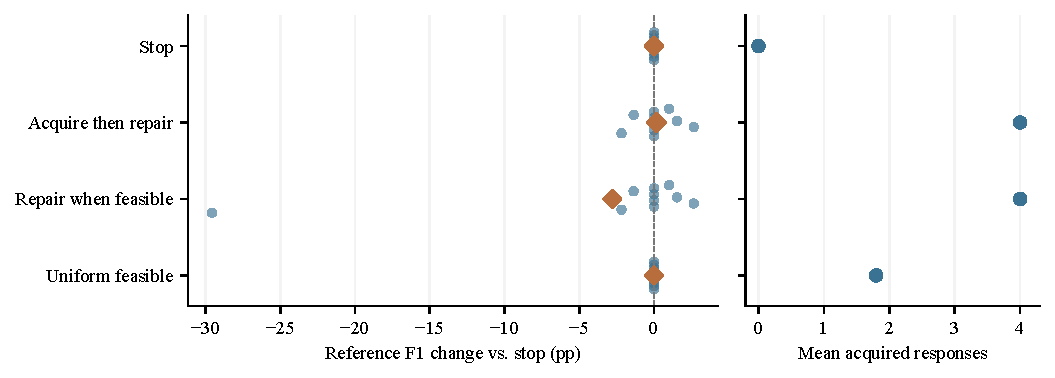
\includegraphics[width=0.94\textwidth]{figure/experiments/docred_source_pilot.pdf}
\caption{Source-rule replay. Dots show ten episode F1 changes from stop; diamonds show their mean. The right panel counts acquired saved responses.}
\label{fig:docred_source_pilot}
\end{figure*}


\paragraph{Second development round.}

Round 2 keeps the same twenty documents, compiler, reward, budget,
and expansion check. Prompts add readable entity names and explain
property direction, historical roles, and absent versus conflicting
evidence. Forty more requests complete with zero transport failures.
Thirty-eight responses pass the fixed parser. They yield 243 type
rules, 14 source-support rules, and zero source-contradiction rules.

Acquire-then-repair and repair-when-feasible both reach 95.69\% reference
F1, compared with 94.42\% for stop. Each removes seven of 31 injected
items and loses zero reference facts. All seven removals use type rules.
The source-repair check ends the two-round study.

The compiler rejects 120 type candidates in round 1 and 257 in round 2
that copy \texttt{allowed or forbidden} instead of choosing one kind.
Both rounds use the fixed parser. The logs retain round 1 reference
losses and round 2 source-rule results.

\begin{figure*}[t]
\centering
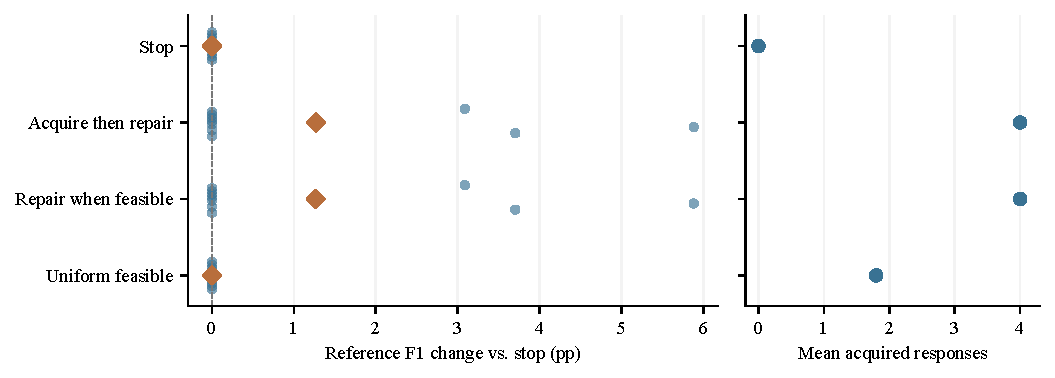
\includegraphics[width=0.94\textwidth]{figure/experiments/docred_source_pilot_round2.pdf}
\caption{Round 2 on the same ten development pairs. Both full schedules reach 95.69\% mean F1 and keep every reference fact. Seven removals use type rules.}
\label{fig:docred_source_round2}
\end{figure*}


\section{New Rule-Execution Test}

\label{app:new_rule_feasibility}

A new fixed protocol uses twenty other development documents.
We take the first ten pairs in development order whose members are absent
from prior pilot lists and response logs. Each pair has a reference graph
and a graph with injected records. There are 226 reference facts and
28 injected items. The test scores controlled reference recovery.

The prompts give exact JSON choice examples and allow at most twenty
rules and three extra sentences. Duplicate keys, invalid choices, or long
lists invalidate the whole response. Candidates then pass the fixed
vocabulary and quote checks. Forty requests use
\texttt{google/gemma-4-26B-A4B-it}, temperature zero, and a 4,000-token
limit. Transport failures and retries are zero. One response exceeds
the rule limit and becomes an empty packet.

The 39 valid responses give 109 allowed and 36 forbidden type rules,
256 source-support rules, and six source-contradiction rules.
All six contradictions come from deletion. The compiler skips 163
insufficient-evidence decisions and rejects nineteen candidates with
quotes absent from the original text.

\begin{table}[t]
\centering
\caption{New rule test on ten document pairs. F1, facts kept (Kept), and packet counts are pair means. Removed injected items (Rem.) and lost reference facts (Lost) are totals. Both-bank schedules give the same final graphs.}
\label{tab:new_rule_feasibility}
\small
\setlength{\tabcolsep}{3pt}
\begin{tabular}{lrrrrr}
\toprule
Schedule & F1 (\%) & Kept (\%) & Rem. & Lost & Packets \\
\midrule
Stop & 94.02 & 100.00 & 0 & 0 & 0.0 \\
Both banks & 96.63 & 98.14 & 17 & 4 & 4.0 \\
Deletion only & 96.63 & 98.14 & 17 & 4 & 2.0 \\
Augmentation only & 94.24 & 100.00 & 1 & 0 & 2.0 \\
Uniform feasible & 95.58 & 100.00 & 8 & 0 & 2.1 \\
\bottomrule
\end{tabular}
\end{table}

The eight fixed schedules are stop, both acquisition orders with immediate
or deferred repair, deletion only, augmentation only, and uniform allowed
actions including stop. Eighty replays agree with all 384 terminal paths.
Random scheduling uses one fixed seed per pair.
Acquire-then-repair leads stop by 2.61 F1 points. The descriptive 95\%
paired-bootstrap interval is $[0.81,4.30]$ from 10,000 draws of ten pairs.
The mean share of reference facts kept is 98.14\%, with four lost facts; the threshold is 99\%.

We remove source-contradiction rules at each pre-edit state to check which
targets lose their flags. This finds three injected-item removals across
two episodes and two reference losses that need source contradictions.
Deletion has sixteen unique injected-item removals compared with
augmentation. Augmentation has zero.

The protocol also checks the best allowed safe schedule, or oracle.
It requires at least 0.5 F1 points over the strongest fixed schedule,
or at least one packet of mean savings at equal quality.
Savings must occur in two or more episodes. A safe path keeps at least
99\% of reference facts in its episode. The oracle uses scorer references
after replay. Its mean F1 is 96.75\%, 0.12 points above deletion alone.
One episode has zero safe paths matching the baseline F1.
The format check passes; the other expansion checks stop this run.
This protocol changes both prompts and documents. Inputs, rules,
traces, and costs are in
\texttt{exps/paper2\_rule\_feasibility\_20261004/}.

\paragraph{Checking lost reference facts.}

Recompiling forty responses and replaying eighty schedules reproduces
the saved outputs. Two reference losses come from forbidden type rules:
$\mathrm{LOC}\!\times\!P150\!\times\!\mathrm{LOC}$ and
$\mathrm{LOC}\!\times\!P37\!\times\!\mathrm{MISC}$.
Two more come from source-contradiction rules for university--country
relations. Both cite the same biography sentence. It mentions both
entities and leaves the country relation unstated.
The biography used for the official-language reference also leaves
the country's official language unstated.

Further family-filter tests use the same banks. Under acquire-then-repair,
removing source contradictions keeps fourteen injected-item removals
and two reference losses, at 96.57\% F1. Removing forbidden type rules
keeps four removals and two losses, at 94.33\% F1. Removing both gives
zero losses and zero repairs, at 94.02\% F1. These filters use public
rule families. The full audit has 320 replays including the original
schedules. The results point to reviewing rules before activation.

\subsection{Rule Approval and Coverage}

\label{app:rule_admission}

Three admission settings replay the same ten document pairs under eight
fixed schedules, giving 240 replays. The first checks source links.
The second requires independent approval from an empty registry.
The third requires a hard-schema mapping from DocRED's coarse types;
this mapping is absent. All 407 candidates pass source-link checks.
The two approval settings keep zero rules, including allowed rules
and support rules.

\begin{table}[t]
\centering
\caption{Rule approval on the same development inputs with acquire-then-repair. Removed counts injected items; lost counts reference facts.}
\label{tab:rule_admission_coverage}
\footnotesize
\setlength{\tabcolsep}{3pt}
\begin{tabular}{lrrrr}
\toprule
Admission & Rules & F1 (\%) & Removed & Lost \\
\midrule
Provenance only & 407 & 96.63 & 17 & 4 \\
Independent approval (empty) & 0 & 94.02 & 0 & 0 \\
Hard schema (no mapping) & 0 & 94.02 & 0 & 0 \\
\bottomrule
\end{tabular}
\end{table}

The eighty source-link traces match saved actions, edits, and rewards.
All-path replay gives 384 terminal paths with source-link checks and
190 for each empty approval setting. Requiring approval keeps all four
reference facts lost in the original run. It also removes all seventeen
injected-item repairs. The automatic-review protocol is fixed;
its model comparison remains a later step. Inputs, decisions, and costs
are in \texttt{exps/paper2\_rule\_verification\_20261008/}.

\section{Fixed Reward-Test Protocol}

\label{app:reward_protocol}

Training uses seeds $20000$--$20009$. For seed $s$ and episode
$e\in\{0,\ldots,249\}$, the environment seed is $100000s+e$.
Separate ridge rollouts use seeds $30000$--$30009$ and the same episode
formula. Development scenarios are $920000$--$920019$.
Test scenarios are $930000$--$930029$. They are disjoint from the ten
earlier action-test scenarios. All use the same 450-document base graph.

The training manifest fixes sources, graph data, penalties, four neural
settings, ridge setup, and statistical comparisons. After forty neural
models, ten ridge fits, and development checks, a second manifest records
model and scorer hashes. The test evaluates all eight policies on the
same thirty scenarios. Ten run-seed means supply paired statistical units.

Policies receive public observations and the current mask.
References supply scoring, and the environment holds restoration records.
Saved initial graphs and node/edge changes rebuild every action log.
Reconstruction checks final scores, remaining errors, masks, reward parts,
costs, and returns under all three penalties.

\subsection{Training and Replay Records}

The reward study fixes sources, costs, seeds, and episode budgets before
training forty neural models and ten ridge baselines.
Development checks cover 1,600 outcomes. A second manifest records all
fifty models and scorer hashes before the test runs. Thirty test
scenarios give 2,400 outcomes. Every predefined policy is retained.
The archive saves initial graphs, each graph change, masks, rewards,
and reference scores. Earlier versions keep their own checkpoints
and results. Training and replay use zero API requests.
The earlier extraction test uses Qwen3.8-27B-no-thinking.
Appendix~\ref{app:prompts} gives historical rule-generation settings.

\section{Earlier Count-Penalty Component Study}

\label{app:impl}

Input order is four graph scores; rule precision, recall, and coverage;
four scaled error counts; budget; and active shares of high- and
low-precision modules. Action order is isolated-node cleanup, duplicate
removal, relation repair, missing-endpoint cleanup, deletion acquisition,
augmentation acquisition, mixed acquisition, and pruning.

This study has sixty trained models and 110 evaluations on scenarios
$900000$--$900009$. DQN, Double DQN, and four component settings use
training seeds $10000$--$10009$, 250 episodes, shared network and replay
settings, and 260-episode exploration decay.
Removing graph features zeros indices 0--3 and 7--10.
Removing rule features zeros indices 4--6 and 12--13.
Indices start at zero. Other inputs and the mask stay available.
The mask also reports which rules allow an action.

The no-mask setting removes action-selection and Bellman masks.
The no-call-penalty setting removes training acquisition cost.
All evaluations use the count penalty, shared costs, and 18 steps.
For AUC, early terminal quality is carried forward to step 18.
The archive retains the older short-action log AUC separately.

Two-sided paired sign randomization uses all $2^{10}$ sign assignments.
Intervals use 10,000 whole-scenario bootstrap draws with seed 42.
Holm correction covers ten comparisons: full Double DQN against
the heuristic and four component settings, for final quality and AUC.
These tests reuse the ten original scenarios.

\begin{table*}[t]
\centering
\caption{Policy scores on ten paired scenarios: mean and sample standard deviation. Calls count simulated acquisition units.}
\label{tab:rl_ablation}
\footnotesize
\setlength{\tabcolsep}{3pt}
\begin{tabular*}{\textwidth}{@{\extracolsep{\fill}}lrrrrrr@{}}
\toprule
Policy & Final quality & AUC$_{18}$ & Calls & Invalid & New errors & Return \\
\midrule
Random valid & $0.9642\pm0.0065$ & $0.9254\pm0.0152$ & 10.2 & 0.0 & 2.9 & 0.3163 \\
Alternating valid & $0.9677\pm0.0007$ & $0.9292\pm0.0020$ & 10.0 & 0.0 & 4.0 & 0.3102 \\
Rule-first valid & $0.9747\pm0.0004$ & $0.9365\pm0.0024$ & 8.0 & 0.0 & 4.6 & 0.3255 \\
Acquire + deficit & $0.9825\pm0.0001$ & $0.9580\pm0.0014$ & 4.0 & 0.0 & 4.8 & 0.3508 \\
DQN & $0.9692\pm0.0037$ & $0.9454\pm0.0079$ & 5.2 & 0.0 & 0.0 & 0.3688 \\
Double DQN & $0.9686\pm0.0034$ & $0.9451\pm0.0096$ & 6.2 & 0.0 & 0.0 & 0.3660 \\
Model-informed lookahead & $0.9711\pm0.0048$ & $0.9516\pm0.0027$ & 5.1 & 0.0 & 0.2 & 0.3750 \\
\bottomrule
\end{tabular*}
\end{table*}


\subsection{Earlier Policy Results}

Count-penalty Double DQN reaches final quality 0.96855 and AUC 0.94514,
with 6.2 acquisition units. Acquire-then-deficit reaches 0.98248 and
0.95797 with four units. Double DQN minus the heuristic is $-0.01392$
for quality and $-0.01283$ for AUC. Both Holm-adjusted $p$ values are
0.0195 (Table~\ref{tab:offline_tests}). DQN reaches quality 0.96920.

Double DQN adds zero violations in ten runs. The heuristic adds 4.8
per run. For $\mathcal R=\sum_{t=0}^{T-1}0.95^t r_t$, their mean
returns are 0.3660 and 0.3508. Section~\ref{subsec:rl_results} shows
that Double DQN avoids relation repair. These returns use the count
penalty. Logs retain each reward part and new error ID.

\begin{figure*}[t]
\centering
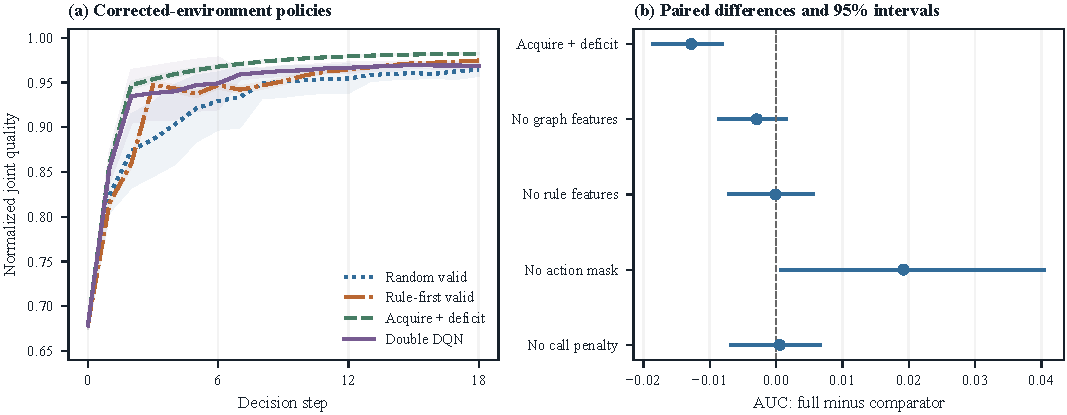
\includegraphics[width=0.98\textwidth]{figure/experiments/math_revision_policy.pdf}
\caption{Earlier count-penalty study on ten reused scenarios. (a) Mean quality with one-standard-deviation bands. Final scores carry forward to step 18. (b) Full Double DQN minus each baseline in AUC, with 95\% paired-bootstrap intervals. Table~\ref{tab:offline_tests} gives adjusted tests.}
\label{fig:rl_convergence}
\end{figure*}

\subsection{Retrained Component Tests}

Ten models per setting train for 250 episodes. Four settings remove
graph features, rule features, the mask, or training acquisition cost.
Feature removal applies in training and evaluation. These settings
retain the mask. The no-mask setting changes action selection and
Bellman targets. The no-call-cost setting changes the training reward.
All evaluations use the same corrected count reward and costs.

\begin{table*}[t]
\centering
\caption{Component tests in the corrected environment. Each setting has ten retrained models.}
\label{tab:offline_ablations}
\footnotesize
\setlength{\tabcolsep}{3pt}
\begin{tabular*}{\textwidth}{@{\extracolsep{\fill}}lrrrrrr@{}}
\toprule
Setting & Final quality & AUC$_{18}$ & Calls & Invalid & New errors & Return \\
\midrule
Double DQN & $0.9686\pm0.0034$ & $0.9451\pm0.0096$ & 6.2 & 0.0 & 0.0 & 0.3660 \\
No graph features & $0.9713\pm0.0041$ & $0.9481\pm0.0028$ & 5.1 & 0.0 & 0.9 & 0.3693 \\
No rule features & $0.9692\pm0.0062$ & $0.9452\pm0.0034$ & 7.6 & 0.0 & 0.5 & 0.3594 \\
No action mask & $0.9480\pm0.0215$ & $0.9259\pm0.0278$ & 4.9 & 10.7 & 0.0 & 0.3430 \\
No call penalty & $0.9659\pm0.0051$ & $0.9446\pm0.0044$ & 8.1 & 0.0 & 0.0 & 0.3596 \\
\bottomrule
\end{tabular*}
\end{table*}


\begin{table*}[t]
\centering
\caption{Full Double DQN minus each baseline. Each interval is a paired-bootstrap 95\% CI. Holm correction covers ten tests.}
\label{tab:offline_tests}
\footnotesize
\setlength{\tabcolsep}{3pt}
\begin{tabular*}{\textwidth}{@{\extracolsep{\fill}}llrrr@{}}
\toprule
Baseline & Metric & Difference & 95\% interval & $p_{\mathrm{Holm}}$ \\
\midrule
Acquire + deficit & Final & -0.01392 & [-0.01604, -0.01205] & 0.0195 \\
Acquire + deficit & AUC & -0.01283 & [-0.01853, -0.00817] & 0.0195 \\
No graph features & Final & -0.00273 & [-0.00601, -0.00007] & 0.8340 \\
No graph features & AUC & -0.00292 & [-0.00862, +0.00151] & 1.0000 \\
No rule features & Final & -0.00068 & [-0.00406, +0.00268] & 1.0000 \\
No rule features & AUC & -0.00008 & [-0.00706, +0.00558] & 1.0000 \\
No action mask & Final & +0.02055 & [+0.00897, +0.03502] & 0.0195 \\
No action mask & AUC & +0.01921 & [+0.00075, +0.04042] & 0.8340 \\
No call penalty & Final & +0.00269 & [-0.00031, +0.00572] & 0.8340 \\
No call penalty & AUC & +0.00053 & [-0.00674, +0.00667] & 1.0000 \\
\bottomrule
\end{tabular*}
\end{table*}


Removing the mask lowers final quality to 0.94800 and gives 10.7 invalid
actions per run. Its quality test has Holm $p=0.0195$; its AUC test has
$p=0.8340$. Graph-feature, rule-feature, and call-cost tests have adjusted
$p>0.05$ across ten comparisons. The mask improves final quality.

Exact paired tests use all $2^{10}$ sign assignments. Holm correction
covers full Double DQN against the heuristic and four component settings
for both scores. Intervals use 10,000 paired bootstrap draws.
Sixty models complete 15,000 training episodes. Earlier checkpoints
keep their original environment version.

\section{Code and Result Files}

\label{app:artifact_index}

Original checkpoints, graph steps, and generation records remain in
their experiment directories.
\texttt{exps/paper2\_offline\_revision/} contains source hashes, forty
checkpoints, training histories, paired action logs, equal-call samples,
rule sources, label checks, and publication scripts. It includes
manuscript-to-result checks and offline replay commands.

\texttt{exps/math\_revision\_20260925/} contains the corrected environment,
sixty checkpoints, full action logs, the shared-profile Paper1 revision,
and the rule interface. It includes a source manifest and replay command.

\texttt{exps/paper2\_reward\_validation/} contains training and test
manifests, forty neural checkpoints, ten ridge models, exploration data,
action logs, paired tests, reconstruction checks, and figure/table scripts.
Its README gives local commands with zero API requests or model downloads.

\texttt{exps/paper2\_rule\_integration/} fixes the raw CSV snapshots,
keeps matching and nonmatching rules, and saves sixteen schedule traces.
Runtime inputs and scorer labels are stored apart. Synthetic interface
tests have their own counts.

\paragraph{Checking all scheduling paths.}

\texttt{exps/papers\_readiness\_20261002/} enumerates every allowed
acquisition, repair, and stop path under four packets and ten steps.
It uses the two development rounds and their twenty shared documents.
References score paths after enumeration.
Table~\ref{tab:offline_loop_ceiling} gives two bounds. The schedule oracle
uses allowed action paths. The relaxed bound can remove each injected
item reached by a stored proposal.

\begin{table}[t]
\centering
\caption{All scheduling paths on the same ten development pairs per round. F1 averages pairs. Oracle scores use reference labels after replay.}
\label{tab:offline_loop_ceiling}
\footnotesize
\begin{tabular}{lrr}
\toprule
Diagnostic & Round 1 & Round 2 \\
\midrule
Feasible terminal paths & 363 & 235 \\
Stop F1 (\%) & 94.42 & 94.42 \\
Executable oracle F1 (\%) & 95.45 & 95.69 \\
Selective-removal upper F1 (\%) & 95.60 & 95.69 \\
Reward-optimal F1 (\%) & 91.63 & 95.69 \\
Oracle correct facts lost & 0 & 0 \\
Oracle injected items removed & 5 & 7 \\
\bottomrule
\end{tabular}
\end{table}


In round 1, the schedule oracle reaches 95.45\% F1. Paths with the
highest proxy reward reach 91.63\%, compared with 94.42\% for stop.
Wrong rules thus make the proxy reward favour lower reference F1.
In round 2, both oracle bounds reach 95.69\%, equal to
acquire-then-repair. Deletion type rules cover all seven removable
injected items. Augmentation and source rules add zero removals.
All-packet repair reaches identical final graphs across acquisition
orders. Discounted returns vary with order. This further development
analysis has 598 terminal paths.

The JSON-contract draft gives legal choices, rule families, candidate
limits, and empty outputs. The unchanged compiler reproduces rules and
rejections for all 80 old responses. Appendix~\ref{app:new_rule_feasibility}
tests this format on other documents. The old rounds retain their
original parser and scores.

\section{Further Repair Tests}

\label{app:supporting_checks}

These tests measure detector coverage, structural repair, and extraction.
Section~\ref{subsec:rl_results} gives policy comparisons.
Section~\ref{subsec:generated_rule_transfer} gives generated-rule effects.

\subsection{Separate Rule-Family Check}

\label{subsubsec:rule_family_final_ablation}

\begin{table}[t]
\centering
\caption{Hand-written family checks scored against stored suite labels. Table~\ref{tab:direct_execution} gives compiled generated patterns.}
\label{tab:rule_family_final_ablation}
\footnotesize
\setlength{\tabcolsep}{3pt}
\begin{tabular*}{\columnwidth}{@{\extracolsep{\fill}}lrrrrr@{}}
\toprule
Detector & TP & FP & FN & Recall & F1 \\
\midrule
Deletion-family & 34 & 0 & 30 & 0.531 & 0.694 \\
Augmentation-family & 30 & 0 & 34 & 0.469 & 0.638 \\
Family union & 64 & 0 & 0 & 1.000 & 1.000 \\
\bottomrule
\end{tabular*}
\end{table}


Hand-written deletion-family checks cover 34 required-step, missing-field,
and specialist defects. Augmentation-family checks cover 30 structural
defects. Their union detects all 64 and flags zero clean records under
the stored labels. The functions directly encode these defect families.
Table~\ref{tab:direct_execution} tests saved generated patterns.

\subsection{Constraint-Checking Baseline}

\label{subsec:shacl_baseline}

The SHACL-style RDF baseline receives unique triples and checks
selected schema shapes. Its inputs contain graph records and shapes.
This test measures the shapes' coverage.

\begin{table}[t]
    \centering
    \caption{SHACL-style structural checks on three domains.}
    \label{tab:shacl_baseline}
    \footnotesize
    \setlength{\tabcolsep}{2pt}
    \begin{tabular*}{\columnwidth}{@{\extracolsep{\fill}}l r r c c@{}}
    \toprule
    Domain & Raw Triples & RDF Dedup. & Removed & $Q$ \\
    \midrule
    Gov. Affairs & 13,892 & 10,771 & 0 & 79.87 \\
    Finance & 2,264 & 539 & 0 & 70.42 \\
    Env. & 2,345 & 378 & 0 & 65.25 \\
    \midrule
    Average & 6,167 & 3,896 & 0 & 71.85 \\
    \bottomrule
    \end{tabular*}
\end{table}

After RDF duplicate removal, all inputs pass the selected shapes.
The baseline removes zero further triples. Its mean quality score is
71.85 under the separate metric. The selected shapes check schema form.
The quality metric also includes source and required-step checks.

\subsection{Deterministic Structural Repair}

\label{subsec:external_benchmark}

A local TNEWS/CLUE test builds a document--category--entity KG from
3,000 balanced news titles across 15 categories. A fixed extractor
builds the graph. We add duplicate triples, invalid relations, and
isolated nodes, then run the repair pipeline. This test uses local
code and zero model or API calls.

\begin{table}[t]
    \centering
    \caption{Local TNEWS/CLUE graph-quality test.}
    \label{tab:tnews_external_benchmark}
    \footnotesize
    \setlength{\tabcolsep}{2pt}
    \begin{tabular*}{\columnwidth}{@{\extracolsep{\fill}}l c c c c@{}}
    \toprule
    Stage & Nodes & Relations & Invalid & $Q$ \\
    \midrule
    Clean extraction & 10,871 & 20,827 & 0.000 & 99.89 \\
    Corrupted KG & 11,414 & 22,909 & 0.050 & 94.93 \\
    Repaired KG & 10,822 & 19,799 & 0.000 & 100.00 \\
    \bottomrule
    \end{tabular*}
\end{table}

Repair removes injected invalid relations, duplicate triples, and isolated
noise nodes. Structural $Q$ rises from 94.93 to 100.00.
The final graph has fewer nodes and relations than the clean extraction.
\texttt{exps/external\_benchmark\_runner.py} generates the report.

\subsection{Model Extraction Test}

\label{subsec:api_llm_benchmark}

The model-extraction test uses 45 TNEWS/CLUE titles across 15 categories
and Qwen3.8-27B-no-thinking. Category labels supply reference values
for category inference. Given title keywords supply weak mention labels.
We score parsing, category accuracy, keyword recall, and structural
filtering.

\begin{table}[t]
    \centering
    \caption{Model extraction on TNEWS/CLUE titles.}
    \label{tab:api_llm_benchmark}
    \footnotesize
    \setlength{\tabcolsep}{2pt}
    \begin{tabular*}{\columnwidth}{@{\extracolsep{\fill}}l c c@{}}
    \toprule
    Metric & Raw LLM KG & Repaired KG \\
    \midrule
    Parse success & 1.000 & --- \\
    Category accuracy & 0.556 & 0.556 \\
    Keyword recall & 0.178 & 0.178 \\
    Documents with triples & 1.000 & 1.000 \\
    Avg. triples / doc & 3.58 & 3.58 \\
    Invalid triple rate & 0.000 & 0.000 \\
    Duplicate triple rate & 0.000 & 0.000 \\
    KG quality score & 100.00 & 100.00 \\
    \bottomrule
    \end{tabular*}
\end{table}

All 45 responses parse. The calls take 1,190.90 seconds.
Every output follows the allowed schema. The filter changes zero triples,
and both input and output structural quality are 100.00.
Category accuracy is 0.556 and keyword recall is 0.178.
These scores point to category choice and missing mentions as targets
for better extraction.

\section{Rule Coverage and Time Records}

\label{app:bridge_coverage}

\subsection{Types and Fixed-Schedule Traces}

The interface in Section~\ref{sec:rule_bridge_method} loads deletion
or augmentation rules, removes unopposed forbidden matches, or stops.
Two acquisition orders with immediate or deferred repair give four
schedules per input. RuleTest-94 and three snapshots give sixteen traces.
All four schedules remove the same ten defects and zero clean records
on RuleTest-94. Late allowed rules and conflicts are zero.
Separate synthetic tests check conflicts and late-allowed rule logging.

Government, finance, and environment snapshots have 17,939, 8,180,
and 151 edge copies. All node types are \texttt{Unknown}.
The 26,270 edges therefore lack required endpoint types. The source audit
checks 51 node CSV files, three document JSONL files, and two extraction
checkpoints. It finds zero traceable types. Enhanced exports use
\texttt{Enhanced} as a processing tag. Export identity requires a
traceable mapping. The runtime skips these records.
Table~\ref{tab:rule_integration_coverage} separates missing types from
zero pattern matches. Appendix~\ref{subsec:shacl_baseline} uses its own
stored inputs.

Both RuleTest-94 matches come from deletion. One allowed rule matches
ten records; one forbidden rule flags ten more. Augmentation matches zero.
All schedules give the same final records. Further scheduling tests
need trusted types and broader useful rule coverage.
Loading one strategy bank reads 4,728 saved responses and uses
zero API requests.

\subsection{Time Details}

\label{app:runtime_details}

The original twenty-model run records 1,278.99 seconds of CPU time and
zero API calls. The sixty-model component study and forty-model reward
study also use zero requests. Ridge adds ten fits from 2,500 random
episodes. Rate-reward component tests add fifty models with zero requests.
The archive gives training and evaluation times. Evaluation includes
policy inference and graph steps. Construction time is excluded.
The model-informed baseline also times copied-state trials.

The 45-document extraction test uses 45 calls and 1,190.90 seconds.
The rule archive has 9,456 successful responses. Complete historical
latency, token, retry, and failure records are absent.
Equal-call tests count candidates per saved successful response.
Scheduling uses simulated acquisition units.
